    \subsection{Eccentricità}
        \begin{frame}{Calcolo dell'eccentricità}
            \begin{columns}
                \column{.4\textwidth}
                    \begin{equation}
                        e = \sqrt{1+\frac{2EL^2}{m_r\alpha^2}}
                    \end{equation}
                    Con
                    \begin{itemize}
                        \item E: energia orbitale*
                        \item L: momento angolare orbitale
                        \item $m_r=\frac{Mm}{m+M}$: massa ridotta del sistema
                        \item $\alpha = F r^2 = GMm$
                    \end{itemize}
                    \small *solo interazione gravitazionale col Sole
                \column{.6\textwidth}
                    \centering
                    \includegraphics[width=.9\textwidth, height=3.75cm]{6_ecc/.jpg}
                    %mettigrafico buggato di mercurio
                    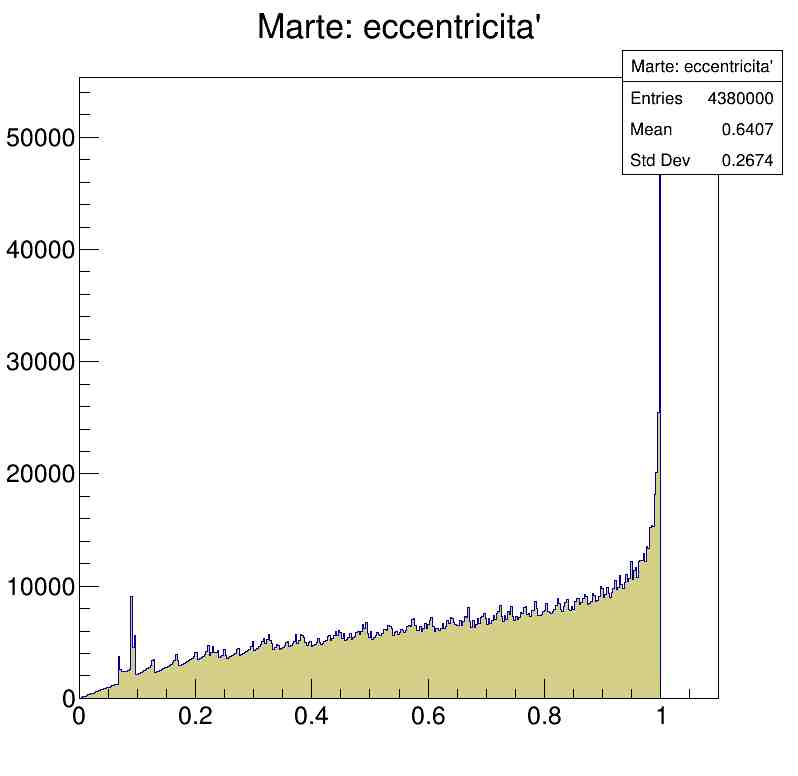
\includegraphics[width=.9\textwidth, height=3.75cm]{6_ecc/mar_ecc_bug.jpg}
                    \label{cfr::bug} 
            \end{columns}
        \end{frame}
        \begin{frame}{Calcolo dell'eccentricità - correzione}
            \begin{columns}
                \column{.4\textwidth}
                    \begin{equation}
                        e = \sqrt{1+\frac{2EL^2}{m_r\alpha^2}}
                    \end{equation}
                    Con
                    \begin{itemize}
                        \item E: energia orbitale*
                        \item L: momento angolare rispetto al sole - eliminiamo la componente di traslazione del sistema
                        \item $m_r=\frac{Mm}{m+M}$: massa ridotta del sistema
                        \item $\alpha = F r^2 = GMm$
                    \end{itemize}
                    \small *solo interazione gravitazionale col Sole
                \column{.6\textwidth}
                    \centering
                    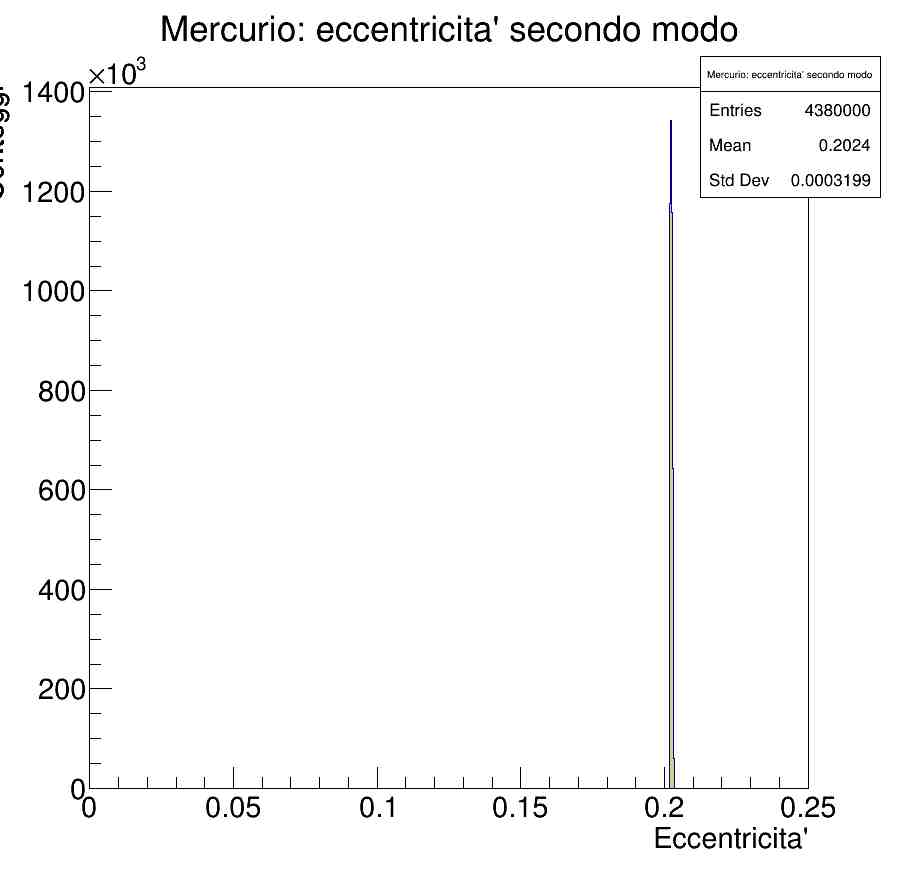
\includegraphics[width=.9\textwidth, height=3.75cm]{6_ecc/mer_ecc_500_3600.jpg}
                    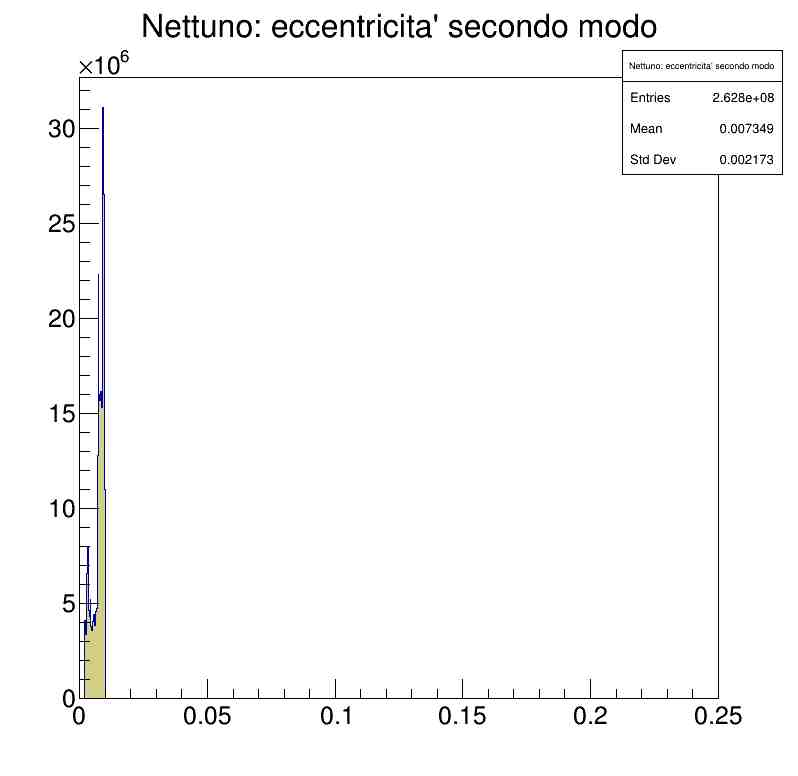
\includegraphics[width=.9\textwidth, height=3.75cm]{6_ecc/net_ecc_500_60.jpg}
                    \label{cfr::bug3} 
            \end{columns}
        \end{frame}
        \begin{frame}{Eccentricità - dipendenza dai parametri}
            \begin{block}{Risultati molto più piccati ma fortemente dipendenti dalle condizioni, non sempre corretti:}
                \begin{itemize}
                    \item Terra e Venere: valori sempre lontani da quelli reali
                    \item Altri pianeti:
                    \begin{itemize}
                        \item Afelio: valori compatibili tra simulazioni con diversi T e deltaT, ma bassi rispetto a quelli reali
                        \item Perielio: valori compatibili tra simulazioni con diversi T e deltaT, ma alti rispetto a quelli reali per quasi tutti i pianeti
                        \item Mix: valori compatibili tra simulazioni con diversi T e deltaT, compatibili anche col valore reale fino a qualche migliaia di anni
                    \end{itemize}
                \end{itemize}               
            \end{block}
            \begin{table}[]
                \centering
                \begin{tabular}{c|ccc|c}
                    500/3600 & Afelio & Prielio & Mix & Reale \\
                    \hline
                    Mercurio & 0.201473 & 0.212235 & 0.202448 & 0.2056 \\
                    Terra & \textbf{0.0119076} &\textbf{ 0.0219439} & 0.0134867 & 0.0167 \\
                    Giove & \textbf{0.0297916} & 0.046467 & 0.0470972 & 0.0484 \\
                    Nettunp & 0.00735812 & \textbf{0.0132255} & 0.00734893 & 0.0086 \\
                \end{tabular}
                %\caption{Caption}
                \label{tab:ecce}
            \end{table}
        \end{frame}